%  ALU_Test.tex
%  <+Last Edited: Thu 17 Apr 2014 15:34:48 BST by seblovett on seblovett-Ubuntu +>

\section{Arithmetic Logic Unit}
\todo[color=cyan, inline]{Include Sub-module tests}
\todo[color=cyan, inline]{Explain tests - what is done}
\todo[color=cyan, inline]{why it is done}
\todo[color=cyan, inline]{How it verifies everything - why it is complete}
\todo[color=cyan, inline]{Show simulation results}

To promote the use of hierarchy within design the ALU is broken down into a number of sub-modules. These have been tested individually to ensure they operate as expected. Then they are combined into a 16-bit ALU without decoder for testing the combination of ALU and LLI slices. As well as more useful shifting tests. Since the LLI slices are either a single multiplexor or wires they will not be tested individually. They will form a part of the ALU Block testing. 

\subsection{ALU Slice}
Testing of this module was broken down into the different ALU functions to be performed: arithmetic, logic and shifting. Control inputs which effect the behaviour of arithmetic operations are SUB and ZeroA. As such tests were run to cover every combination of A, B and CIn for addition, subtraction and both with ZeroA enabled. The test results are shown in Figure~\ref{fig:ALUSliceRes}. For subtraction tests, because additional logic for handling subtraction carrys is within the decoder, the outputted response shows inverted Cin and Borrow signals. For both of the last two groupings input A is active during the length of testing, which shows that zero is used when ZeroA is active. Whilst testing logic operations, each gate is tested for its full range of input combinations to show correct operation. The output of these tests are shown in Figure~\ref{fig:ALUSliceRes}. Testing of the shifting capabilities involved setting all inter-slice inputs high with the input A held low. Then for each case of: left, right and left with B input shifting, different immediate signals were set to observe the propagation of bits through the slice. If a bit in the 4-bit immediate controlling the amount to shift is high, a 1 would be outputted in the next adjacent bit of the output. This is OutLeft for left shifting of OutRight for right shifting as shown in Figure~\ref{fig:ALUSliceRes}. 
\todo[inline]{check explaination}

\begin{figure}[h]
	\centering
	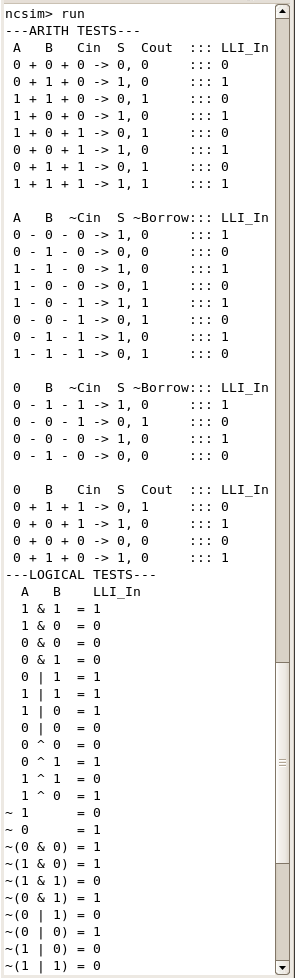
\includegraphics[scale=0.72]{results/ALUSliceA.png}
	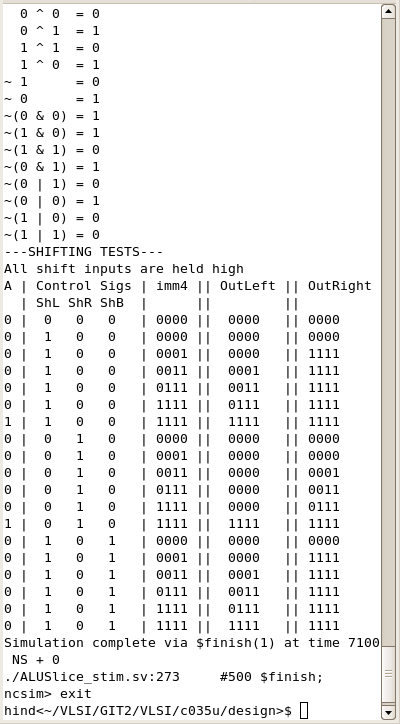
\includegraphics[scale=0.72]{results/ALUSliceB.png}
	\caption{Test Results for ALUSlice}
	\label{fig:ALUSliceRes}
\end{figure}
\todo[inline]{Adjust shifting output to include aluout}

\subsection{ALU Decoder}
The main testing of the ALU decoder module requires ensuring a correct response to each possible opcode. Secondary testing covers the flag calculation circuitry and the bit to input for right shifting operations. The test results are shown in Figure~\ref{fig:ALUDecoderRes}, where each line indicates what input changed and which control and flag outputs are active as a result. 

Basic tests run through each opcode and ensure the outputted signals are as expected from Table~\ref{tab:contrOuts}. The signal {\bf \it CIn\_Slice} is the carry input to the top ALU slice after CIn has been influenced by UseC and SUB. While the signal {\bf \it ShiftIn} is the bit used for right shifting accounting for the current operation and data sign. Subsequent tests ensure correct flags and shifting signals. 

\begin{figure}[h]
	\centering
	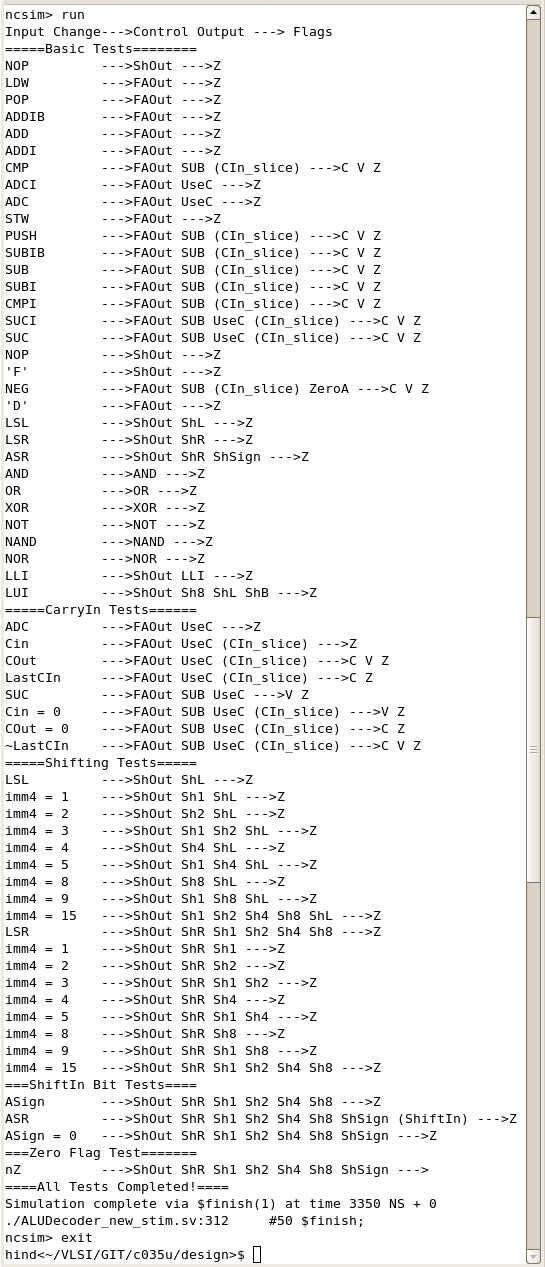
\includegraphics[scale=0.56]{results/ALUDecoder.png}
	\caption{Test Results for ALUDecoder}
	\label{fig:ALUDecoderRes}
\end{figure}

\subsection{ALU Block}
Testing of 16 connected slices involved a similar approach to an individual slice, but with full 16 bit values. Arithmetic used two random value inputs combined with the possible carry in values. Logic tests are no different. Whilst shifting tests show the correct operation on a given quantity with an equivalent 8-bit left shifting operation for LUI. The LLI module also shows correct concatenation of both inputs. The test results are shown in Figure~\ref{fig:ALUBlockRes}.

\begin{figure}[h]
	\centering
	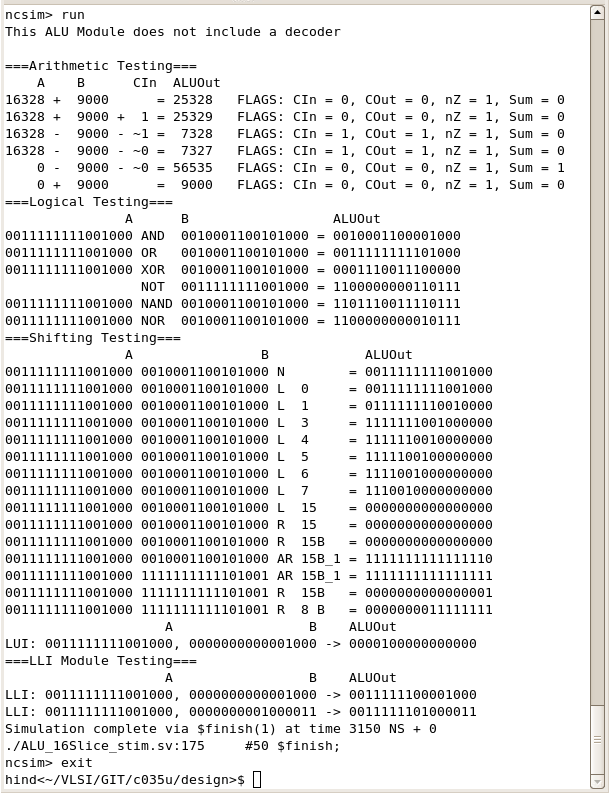
\includegraphics[scale=0.72]{results/ALUBlock.png}
	\caption{Test Results for 16 Slice Block}
	\label{fig:ALUBlockRes}
\end{figure}
